%!TEX root = project.tex

\chapter*{About this project}
\paragraph{Abstract}
A brief description of what the project is, in about two-hundred and fifty words.

\paragraph{Authors}
Explain here who the authors are.



\chapter{Introduction}
The main objective for this project was to create a project that displayed the skills that we have developed throughout our the four years we have spent here at GMIT. For this project I hope to create a web application that helps the user find basic gym exercises based on the sports they play. For example if the user were to select rugby exercises, the application will display a list of exercises focused on the  upper body.

I decided to spend a lot of time thinking about which technologies would be suitable to create this project. During this time, I conducted research on using technologies such as Java and HTML for the front-end. The reasoning behind this would be that I had used these technologies throughout my time in GMIT and that I was very familiar with them. I also thought of using a mySQL database. The reasoning for this is that I had used this in many projects , especially my previous year in college. I chose not to use these technologies as I wanted to test myself and use technologies that I was not familiar with and see how I would get on.

The technologies that I have chosen to develop this project are React for the front-end, MongoDB to store all of the exercises and the Meteor Platform for developing the web application. I will go into greater detail, regarding the technologies used later in the 'Technology Review' section of this dissertation.

\chapter{Context}
\begin{itemize}
\item Provide a context for your project.
\item Set out the objectives of the project
\item Briefly list each chapter / section and provide a 1-2 line description of what each section contains.
\item List the resource URL (GitHub address) for the project and provide a brief list of the main elements at the URL.
\end{itemize}

\section{Filler}
Lorem ipsum dolor sit amet, consectetur adipiscing elit. Etiam mi enim, interdum ut elit lobortis, bibendum tempus diam. Etiam turpis ex, viverra tristique finibus nec, feugiat at metus. Curabitur tempus gravida interdum. Donec ac felis a lorem scelerisque elementum. Vestibulum sit amet gravida tortor, a iaculis orci. Nam a molestie augue. Curabitur malesuada odio at mattis molestie. In hac habitasse platea dictumst. Donec eu lectus eget risus hendrerit euismod nec at orci. Praesent porttitor aliquam diam, eu vestibulum nisl sollicitudin vel. Nullam sed egestas mi.

Quisque vel erat a justo volutpat auctor a nec odio. Sed rhoncus augue sit amet nisl tincidunt, vitae cursus tellus efficitur. Class aptent taciti sociosqu ad litora torquent per conubia nostra, per inceptos himenaeos. Pellentesque et auctor dui. Fusce ornare odio ipsum, et laoreet mi molestie sed. Cras at massa sit amet ipsum gravida aliquam. Nulla suscipit porta imperdiet. Fusce eros neque, bibendum sit amet consequat non, pulvinar quis ipsum.

\subsection{More filler}
Donec fermentum sapien ac rhoncus egestas. Nullam condimentum condimentum eros sit amet semper. Nam maximus condimentum ligula. Praesent faucibus in nisi vitae tempus. Sed pellentesque eleifend ante, ac malesuada nibh dapibus nec. Phasellus nisi erat, pulvinar vel sagittis sed, auctor et magna. Quisque finibus augue elit, consequat dignissim purus mollis nec. Duis ultricies euismod tortor, nec sodales libero pellentesque et. Interdum et malesuada fames ac ante ipsum primis in faucibus.

Donec id interdum felis, in semper lacus. Mauris volutpat justo at ex dignissim, sit amet viverra massa pellentesque. Suspendisse potenti. Praesent sit amet ipsum non nibh eleifend pretium. In pretium sapien quam, nec pretium leo consequat nec. Pellentesque non dui lacus. Aenean sed massa lacinia, vehicula ante et, sagittis leo. Sed nec nisl ac tellus scelerisque consequat. Ut arcu metus, eleifend rhoncus sapien sed, consequat tincidunt erat. Cras ut vulputate ipsum.

Curabitur et efficitur augue. Proin condimentum ultrices facilisis. Mauris nisi ante, ultrices sed libero eget, ultrices malesuada augue. Morbi libero magna, faucibus in nunc vitae, ultricies efficitur nisl. Donec eleifend elementum massa, sed eleifend velit aliquet gravida. In ac mattis est, quis sodales neque. Etiam finibus quis tortor eu consequat. Nullam condimentum est eget pulvinar ultricies. Suspendisse ut maximus quam, sed rhoncus urna.

\section{Filler}
Phasellus eu tellus tristique nulla porttitor convallis. Vestibulum ac est eget diam mollis consectetur. Donec egestas facilisis consectetur. Donec magna orci, dignissim vel sem quis, efficitur condimentum felis. Donec mollis leo a nulla imperdiet, in bibendum augue varius. Quisque molestie massa enim, vitae ornare lacus imperdiet non. Donec et ipsum id ante imperdiet mollis. Nullam est est, euismod sit amet cursus a, feugiat a lectus. Integer sed mauris dolor.

Mauris blandit neque tortor, consequat aliquam nisi aliquam vitae. Integer urna dolor, fermentum ut iaculis ut, semper eu lacus. Curabitur mollis at lectus at venenatis. Donec fringilla diam ac risus imperdiet suscipit. Aliquam convallis quam vitae turpis interdum, quis pharetra lacus tincidunt. Nam dictum maximus lectus, vitae faucibus ante. Morbi accumsan velit nec massa tincidunt porttitor. Nullam gravida at justo id viverra. Mauris ante nulla, eleifend vitae sem vitae, porttitor lobortis eros.

Cras tincidunt elit id nisi aliquam, id convallis ex bibendum. Sed vel odio fringilla, congue leo quis, aliquam metus. Nunc tempor vehicula lorem eu ultrices. Curabitur at libero luctus, gravida lectus sed, viverra mi. Cras ultrices aliquet elementum. Pellentesque habitant morbi tristique senectus et netus et malesuada fames ac turpis egestas. Sed metus ante, suscipit sit amet finibus ut, gravida et orci. Nunc est odio, luctus quis diam in, porta molestie magna. Interdum et malesuada fames ac ante ipsum primis in faucibus. Mauris pulvinar lacus odio, luctus tincidunt magna auctor ut. Ut fermentum nisl rhoncus, tempus nulla eget, faucibus tortor. Suspendisse eu ex nec nunc mollis pulvinar. Nunc luctus tempus tellus eleifend porta. Nulla scelerisque porttitor turpis porttitor mollis.

Duis elementum efficitur auctor. Nam nisi nulla, fermentum sed arcu vel, posuere semper dui. Fusce ac imperdiet felis. Aenean quis vestibulum nisl. Integer sit amet tristique neque, at suscipit tortor. Morbi et placerat ante, vel molestie dui. Vivamus in nibh eget massa facilisis accumsan. Nunc et purus ac urna fermentum ultrices eget sit amet justo. Class aptent taciti sociosqu ad litora torquent per conubia nostra, per inceptos himenaeos. Cras elementum dui nunc, ac tempor odio semper et. Ut est ipsum, sollicitudin eleifend nisl eu, scelerisque cursus nunc. Nam at lectus vulputate, volutpat tellus vel, pharetra mauris. Integer at aliquam massa, at iaculis sem. Morbi nec imperdiet odio. In hac habitasse platea dictumst.

Mauris a neque lobortis, venenatis erat ut, eleifend quam. Nullam tincidunt tellus quis ligula bibendum, a malesuada erat gravida. Phasellus eget tellus non risus tincidunt sagittis condimentum quis enim. Donec feugiat sapien sit amet tincidunt fringilla. Vivamus in urna accumsan, vehicula sem in, sodales mauris. Aenean odio eros, tristique non varius id, tincidunt et neque. Maecenas tempor, ipsum et sollicitudin rhoncus, nibh eros tempus dolor, vitae dictum justo massa in eros. Proin nec lorem urna. In ullamcorper vitae felis sit amet tincidunt. Maecenas consectetur iaculis est, eu finibus mi scelerisque et. Nulla id ex varius, ultrices eros nec, luctus est. Aenean ac ex eget dui pretium mattis. Ut vitae nunc lectus. Proin suscipit risus eget ligula sollicitudin vulputate et id lectus.


\chapter{Methodology}
About one to two pages.
Describe the way you went about your project:
\begin{itemize}
\item Agile / incremental and iterative approach to development. Planning, meetings.
\item What about validation and testing? Junit or some other framework.
\item If team based, did you use GitHub during the development process.
\item Selection criteria for algorithms, languages, platforms and technolo-gies.
\end{itemize}
Check out the nice graphs in Figure \ref{tikz:graphs}, and the nice diagram in Figure \ref{tikz:mydiagram}.

\begin{figure}
  \centering
  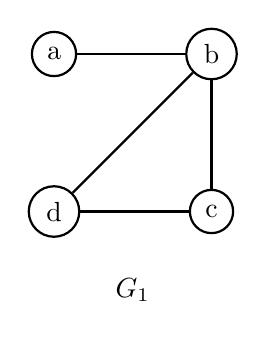
\begin{tikzpicture}
  \begin{scope}[every node/.style={circle,thick,draw}]
  \node (a) at (0,2) {a};
  \node (b) at (2,2) {b};
  \node (c) at (2,0) {c};
  \node (d) at (0,0) {d};
  \end{scope}
  \begin{scope}[every edge/.style={draw=black,thick}]
  \path (a) edge (b);
  \path (b) edge (c);
  \path (b) edge (d);
  \path (c) edge (d);
  \end{scope}
  \node () at (1,-1) {$G_1$};
  \end{tikzpicture}
  \hspace{1.5cm}
  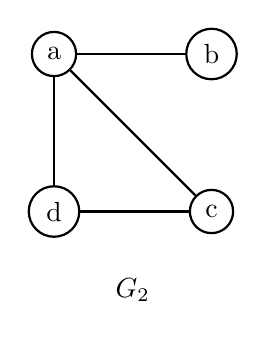
\begin{tikzpicture}
  \begin{scope}[every node/.style={circle,thick,draw}]
  \node (1) at (0,2) {a};
  \node (2) at (2,2) {b};
  \node (3) at (2,0) {c};
  \node (4) at (0,0) {d};
  \end{scope}
  \begin{scope}[every edge/.style={draw=black,thick}]
  \path (1) edge (2);
  \path (1) edge (3);
  \path (1) edge (4);
  \path (3) edge (4);
  \end{scope}
  \node () at (1,-1) {$G_2$};
  \end{tikzpicture}
  \caption{Nice pictures}
  \label{tikz:graphs}
\end{figure}


\begin{figure}
  \centering
  \begin{tikzpicture}[node distance=6cm]
  \node (a) [rect] {A Big Blue Block};
  \node (b) [oval, right of=a] {And His Oval Friend};
  \draw [line] (a) -- (b);
  \end{tikzpicture}
  \caption{Nice pictures}
  \label{tikz:graphs}
\end{figure}


\chapter{Technology Review}
For this part of the dissertation, I will talking about the technologies in which I incorporated into my project. I thought about the many technologies out there which I could use. For my previous final year project last year I decided to use Java to develop the front-end and used an SQL database to store information. This year for this current final year project I decided to use React for the front end. The reasoning behind this is because React has gotten very popular over the last few years. I really wanted to learn how exactly it compares to other languages used for front end programming. For the back end of the project I decided to use Meteor.


\section{React}
The main reasoning for picking React as the main language I used for this project is because I had never used it prior to this project and that it has become so popular over the last few years. React is  a JavaScript library for building user interfaces. It is maintained by Facebook and a community of individual developers and companies[1]. One of the primary features of React is components. Components allow you to split the UI into independent, reusable pieces and think about each piece in isolation-\cite{Components}. Components are the building blocks of a React application. Components are mostly JavaScript classes or functions that accept inputs optionally. A code example of a React component which displays Hello World would look like the following :
\begin{center}    
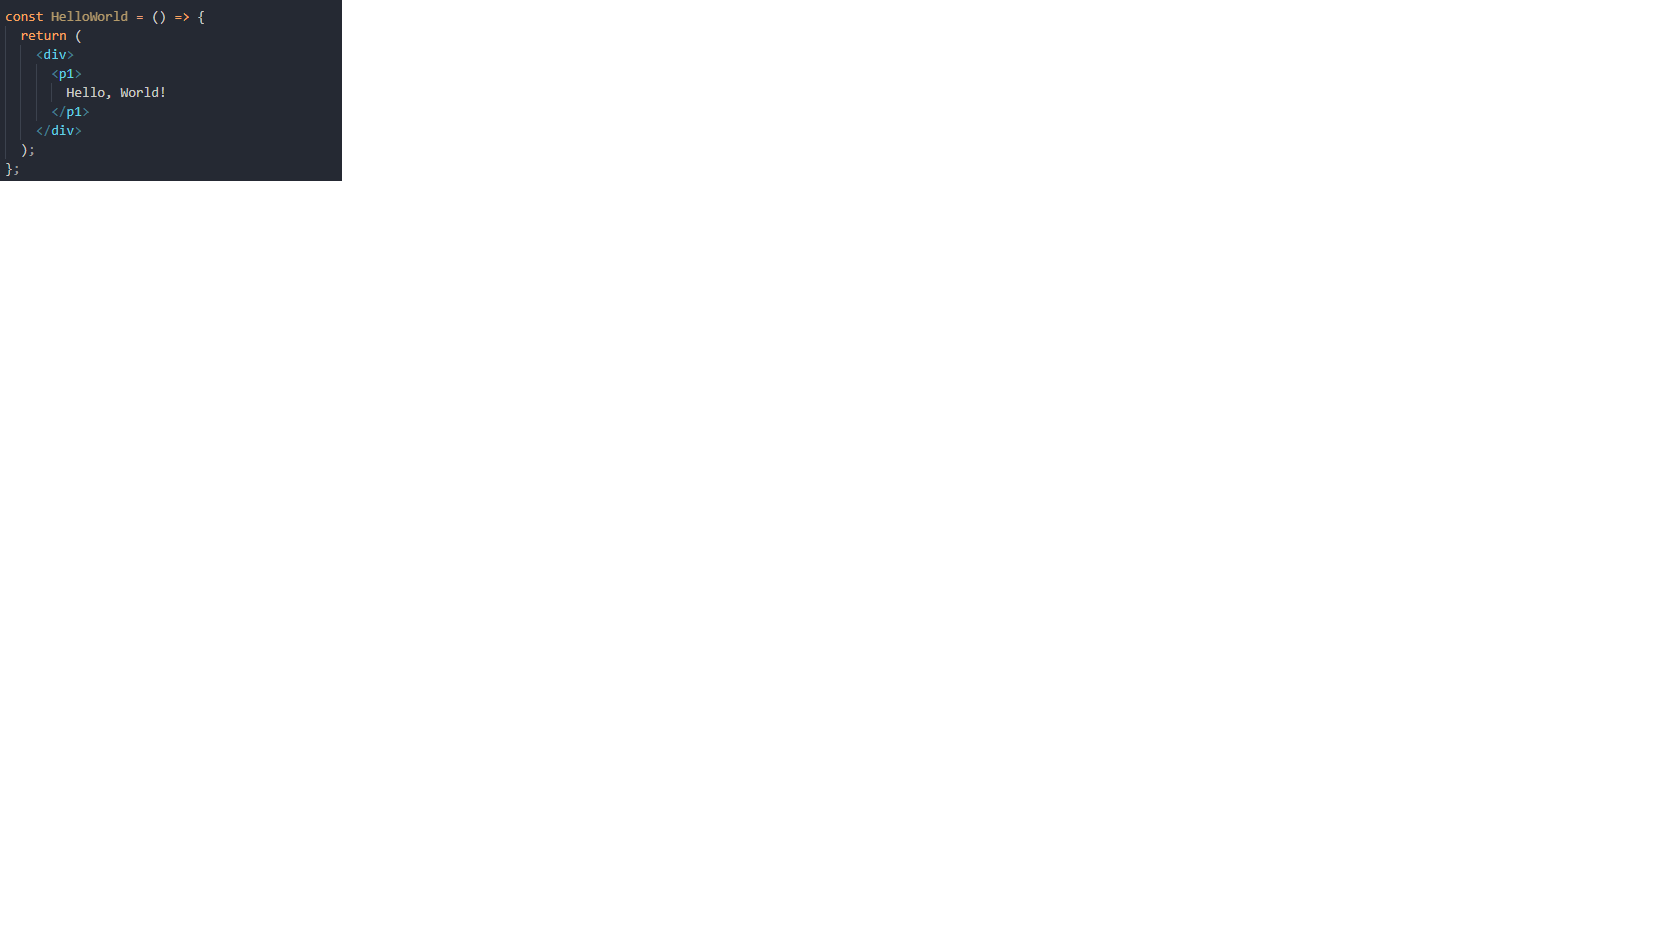
\includegraphics{img/component.png}
\end{center}

In this example you can see that I created a constant called 'HelloWorld', that returns a function in which it prints out 'Hello, World!"

If I then wanted to use this function I would have to put it in a render function which would look like the following:
\begin{center}    
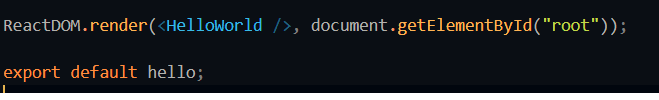
\includegraphics{img/hello.png}
\end{center}

\section{MongoDB}
MongoDB is a cross-platform document oriented database program. Classified as a NoSQL datbase program, MongoDB uses JSON like documents with schemata\cite{MongoDB}. The main reasoning for using a Mongo database for this project was because I had never used it within a project itself before. They only previous experience that I had with Mongo was a module which I did in my second year of my studies here at GMIT. However throughout this module, we only really covered the basic concepts of the databases such as creating a collection, inserting a document into a collection and deleting them. While doing my research I debated on using an SQL database instead of Mongo. The main reasoning behind my choice to use mongo, was that I had already used SQL databases many times in the past and that I wanted to challenge myself and try something new.

The main differences between a Mongo database and a mySQL database would be:

\begin{itemize}
  \item In a Mongo database, data is represented in a collection of JSON documents, while in a SQL database, data is represented in tables and rows.
  \item Another difference would be that mySQL databases supports atomic transactions. This means you can have multiple operations within a transaction and you can roll back if you have a single operation. MongoDB does not support atomic transactions.
  \item Finally, when using MongoDB, you are not responsible for defining the schema. All you have to do is simply drop in the documents that you wish to store. In a SQL database, you have t define the tables and columns before you try to store anything.
\end{itemize}

\section{Meteor}
Meteor or MeteorJS is a free open-source isomorphic JavaScipt web framework writte using Node.js. Meteor allows for rapid prototyping and produces cross-platform code \cite{Meteor}.
The main features of Meteor would include:

\begin{itemize}
    \item Both the back-end and the front-end are wrote in JavaScript.
    \item It automatically applies Node.js in the back end.
    \item It automatically applies MongoDB for the users database.
    \item It provides a library of key packages that most applications will require.
    \item 
\end{itemize}

When deciding on what type of back-end I waned to use for this project, I originally had the idea of using React's back-end as I was writing the majority of the code in React. However I came into issues with deploying my app to server using React's methods, which then lead me on to see what other back-end pieces of technology I could use. I then came into contact with Meteor. The main fact as to why I chose this is because I didn't see much back-end technologies that supported react in the research stages of the project and Meteor seemed to have everything I needed to complete the project.

\section{CSS}
Cascading Style Sheets also known as CSS is a styling sheet language of a document written in a markup language such as HTML. CSS is designed to enable separation of presentation and content including layouts, fonts and colours\cite{CSS}.

Using CSS, in my opinion is probably the most well known method of styling code. I was first introduced to it in my first year of studies here at GMIT, where we learned the basics such as changing the background of a simple HTML page and styling lists etc. I decided to use it in this project as I thought it could make the application more appealing which in my opinion, it did just that. 

The following is an example of how I used CSS with my project. The image below shows a constant that prints out a list of exercises. Within the style tag you can see that I set background colour, text alignment, font type, font size, margin and the type of border:


\begin{center}    
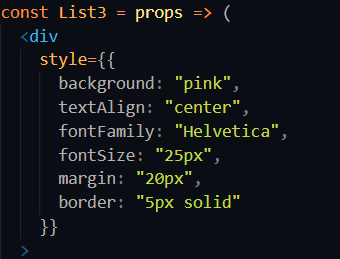
\includegraphics{img/css.png}
\end{center}

\section{Bootstrap}
Bootstrap is an open source toolkit for developing with HTML, CSS and JavaScript\cite{Bootstrap}. It is a free front-end framework that includes design template for typography, forms, buttons, tables, navigation and images.

I decided to use Bootstrap in my project as I think it adds massively to the front-end side of any application. I used it for making simple buttons look more appealing to the user. Bootstrap is very easy to use. The method in which I used to integrate bootstrap with my application was that I  firstly installed it onto my machine by using the following command on the command prompt: 

\begin{lstlisting}
npm install --save bootstrap
\end{lstlisting}

I then proceed to import the downloaded libraries to my project. This was done by including the following line of code on the file that I wished to use bootstrap on:

\begin{lstlisting}
import 'bootstrap/dist/css/bootstrap.css';
\end{lstlisting}

I used Bootstrap throughout the project. An example of where I used it woud be the home page where I used it to style the buttons. Below is an image of the buttons described above:

\begin{center}    
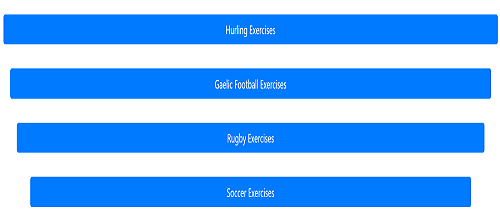
\includegraphics{img/button.png}
\end{center}

\section{Visual Studio Code}
Visual Studio Code is a source code editor developed by Microsoft for Windows, Linux and macOS\cite{Visual} It is a very popular code editor due to its many appealing features. These features include:

\begin{itemize}
\item It includes support for debugging.
\item Git can be used within the software.
\item It has Syntax highlighting.
\item It has code re factoring.
\item It has customizable themes.
\end{itemize}

For this project, I used Visual Studio code to write all of the React and CSS code. The reasoning of this is because I have been using this program over the last few years and in my opinion is the best text editor out there at this point in time due to its many features such as the ones listed above.

\section{Git}
Git is a distributed version control system for tracking changes in source code during software development\cite{Git}. Git is used to track the progress of projects. 

It does this by creating a local repository of your project on your machine. To start a local repository with git, all you have to do is navigate to your project folder and simply type:

\begin{lstlisting}
git init
\end{lstlisting}

This then creates a local repository on your machine. If you wanted to commit a change to the project you can by simply adding your changes to the project by using the following command:

\begin{lstlisting}
git add .
\end{lstlisting}

This command adds all of the changes that it can find in the project folder and add it to the local repository. If you then wanted to push these changes to GitHub, you must first add a remote origin to your local repository. This is done by using the following command:

\begin{lstlisting}
git remote add origin https://github.com/user/Project-name.git
\end{lstlisting}

The command above would link the local repository to a repository on GitHub which then you coud push all of the changes to by using the command below:

\begin{lstlisting}
git push -u origin master
\end{lstlisting}


\section{GitHub}
GitHub is  a web-based hosting service for version control using Git. It offers all of the distributed version control and source code management functionality of Git also and adds its own features\cite{GitHub}.

I used both Git and GitHub throughout this project as it was a requirement. Everytime that I had made a major change in the project I committed it and pushed the changes to my repository on GitHub which can be found here:

\begin{lstlisting}
https://github.com/CathalRyan96/Project-Year-4
\end{lstlisting}

\section{Cmder}
Cmder is a pre-configured software package that provides you with an appealing terminal emulator\cite{Cmder}. Cmder is very similar to the Command Prompt Terminal window that is pre-installed on most machines however it also has many additional features as well.

These features include:
\begin{itemize}
\item Git and all of its commands are already installed onto it, which saves you from downloading Git onto your machine.
\item You can use Unix commands whilst using it. Commands such as ls, rm and chmod.
\item It is very portable. What I mean by saying this is that you can upload it on to any cloud file storing websites such as Dropbox or Google Drive.

\end{itemize}

I used Cmder throughout the project, mainly for my use of Git. I also used it when deploying my application to the local host. I did this by navigating to my project folder and entering the command "Meteor", which can be seen in the image below.

\begin{center}    
  \includegraphics{img/prompt1.png}
  \end{center}
  
  \section{LaTeX}
  LaTeX is a document preparation system. It provides features designed for the production of technical and scientific documentation\cite{LaTeX}. 
  
  I had only used LaTeX once before last semester in the "Research Methods" module in which we had to write a Literature Review in LaTeX. It was also recommended by our lecture to use it as they had already created a template from where we could start from.
  
  I enjoyed using LaTeX as in my opinion styles documents in a much more appealing way rather than using just plain text in programs such as Microsoft Word.
  
  \section{Heroku}
  Heroku is a cloud platform service that supports many programming languages. It is one of the first cloud platforms as it has been in development since 2007. Back then it only supported the programming language called Ruby. However as of now it supports many languages such as Java, Node.js, Scala, Python and PHP\cite{Heroku}.
  
  For this project I deployed my application to Heroku. This was probably one of the most challenging parts of the project. I say this because, I had a lot of issues regarding connecting my Mongo datbase to my application on the cloud. After a lot of testing I finally came to the conclusion of hosting my database on a cloud service known as mLab. Here I created the collections that were present in my local database and connected it to my Heroku Application. As of now most of my application is being deployed on heroku, however some parts such as the about page are not appearing correctly and I am currently trying to figure out why I am getting this error. The application deployed on heroku can be found here:
  
  https://cryanfyp.herokuapp.com/
  
  
  \section{mLab}
  mLab is a fully managed cloud database service that hosts MongoDB databases. mLab runs on cloud providers such as Amazon, Google and Microsoft Azure.
  
  I used mLab to host my database in order for it to connect to my Heroku Application. I did this by creating the collections and documents which were present in my local database and used the Mongo URI to connect it to my Heroku application. 
  
  Images of the collections in the database  on mLab can be seen below:
  \begin{center}    
  \includegraphics{img/mongoC.png}
  \end{center}
  
  Image of an example of a document in the database on mLab can be seen below:
  \begin{center}    
  \includegraphics{img/info.png}
  \end{center}
  

\chapter{System Design}
As many pages as needed.
\begin{itemize}
\item Architecture, UML etc. An overview of the different components of the system. Diagrams etc… Screen shots etc.
\end{itemize}

\begin{table}[h]
  \centering
  \begin{tabular}{x{2cm}p{3cm}}
    \toprule \\
    Column 1 & Column 2 \\
    \midrule \\
    Rows 2.1 & Row 2.2 \\
    \bottomrule
  \end{tabular}
  \caption{A table.}
  \label{table:mytable}
\end{table}

\chapter{System Evaluation}
As many pages as needed.
\begin{itemize}
\item Prove that your software is robust. How? Testing etc. 
\item Use performance benchmarks (space and time) if algorithmic.
\item Measure the outcomes / outputs of your system / software against the objectives from the Introduction.
\item Highlight any limitations or opportuni-ties in your approach or technologies used.
\end{itemize}

\chapter{Conclusion}
About three pages.

\begin{itemize}
\item Briefly summarise your context and ob-jectives (a few lines).
\item Highlight your findings from the evalua-tion section / chapter and any opportuni-ties identified.
\end{itemize}

